\documentclass{report}

% Load preamble
\newcommand{\course}[1]{\newcommand{\courseloc}{#1}}

\usepackage{amsmath,amssymb,amsfonts,mathtools,amsthm}
\usepackage{mathrsfs}
\usepackage{booktabs, emptypage, subcaption, multicol}
\usepackage{braket, bm, lipsum, systeme}
\usepackage{hyperref,theoremref}
\hypersetup{
  pdftitle={assignment},
  colorlinks=true, linkcolor=doc!90,
  bookmarksnumbered=true,
  bookmarksopen=true
}
\usepackage[T1]{fontenc}
\usepackage{anyfontsize}
\usepackage{lmodern}
\usepackage{graphicx}
\usepackage{import}
\usepackage{transparent}
\usepackage{float}
\usepackage[tmargin=2cm,rmargin=1in,lmargin=1in,margin=0.85in,bmargin=2cm,footskip=.4in]{geometry}
\usepackage[shortlabels]{enumitem}
\usepackage[dvipsnames]{xcolor}
\usepackage{xfrac}
\usepackage{comment}
\let\mathbf\relax
\usepackage[varbb]{newpxmath}
\usepackage[most,many,breakable]{tcolorbox}
\usepackage{varwidth}
\usepackage{nameref}
\usepackage[ruled,vlined,linesnumbered]{algorithm2e}
\usepackage{chngcntr}
\usepackage{import}
\usepackage{xifthen}
\usepackage{pdfpages}
\usepackage{transparent}
\usepackage{xparse}
\usepackage{pgffor}
%\usepackage{emoji}
\usepackage{stmaryrd}
\usepackage{listings}
\usepackage{siunitx}
\usepackage{tikz, tikz-cd, tikz-3dplot, tikzsymbols}
\usetikzlibrary{intersections, angles, quotes, calc, positioning, arrows.meta}
\usepackage{pgfplots}
\pgfplotsset{compat=1.13}
\usepackage{thmtools}
\usepackage[framemethod=TikZ]{mdframed}
\usepackage{etoolbox}
\usepackage{xifthen} 
\usepackage{titlesec}
\usepackage[dotinlabels]{titletoc}
\usepackage{fancyhdr}
\usepackage{marginnote}
\usepackage{witharrows}
\usepackage{scalerel}
\usepackage[usestackEOL]{stackengine}
\usepackage[linguistics]{forest}
\usepackage{array}
\usepackage[export]{adjustbox}
\usepackage{multirow}
\usepackage{tabularx}
\usepackage{extarrows}
\usepackage[ 
backend=biber,
backref=true,
style=numeric,
sortcites=true,
sorting=none,
defernumbers=true
]{biblatex}
\usepackage{xurl}
\usepackage[makeroom]{cancel}
\usepackage{bookmark}
\usepackage{tensor}
\usepackage{derivative}
\usepackage{annotate-equations}
\usepackage{dashbox}
\usepackage{nicematrix}
\usepackage{ytableau}
\usepackage{tabularray}
\usepackage{xpatch}





%=================================
%= TikZ things customized        =
%=================================


\newcommand\mycommfont[1]{\footnotesize\ttfamily\textcolor{blue}{#1}}
\SetCommentSty{mycommfont}
\newcommand{\incfig}[2]{%
    \def\svgwidth{#1\columnwidth}
    \import{./figures/}{#2.pdf_tex}
}

\graphicspath{{./figures/}}
\pdfsuppresswarningpagegroup=1







\usepackage{tikzsymbols}
\tikzset{
	symbol/.style={
			draw=none,
			every to/.append style={
					edge node={node [sloped, allow upside down, auto=false]{$#1$}}}
		}
}
\tikzstyle{c} = [circle,fill=black,scale=0.5]
\tikzstyle{b} = [draw, thick, black, -]
\tikzset{
    vertex/.style={
        circle,
        draw,
        minimum size=6mm,
        inner sep=0pt
    }
}

%\tikzset{
%    force/.style={thick, {Circle[length=2pt]}-stealth, shorten <=-1pt}
%}

%%%%%%%%%%%%%%%%%%%%%%%%%%%%%%
% SELF MADE COLORS
%%%%%%%%%%%%%%%%%%%%%%%%%%%%%%

\definecolor{doc}{RGB}{0,60,110}
\definecolor{myg}{RGB}{56, 140, 70}
\definecolor{myb}{RGB}{45, 111, 177}
\definecolor{myr}{RGB}{199, 68, 64}
\definecolor{mytheorembg}{HTML}{F2F2F9}
\definecolor{mytheoremfr}{HTML}{00007B}
\definecolor{mylemmabg}{HTML}{FFFAF8}
\definecolor{mylemmafr}{HTML}{983b0f}
\definecolor{mypropbg}{HTML}{f2fbfc}
\definecolor{mypropfr}{HTML}{191971}
\definecolor{myexamplebg}{HTML}{F2FBF8}
\definecolor{myexamplefr}{HTML}{88D6D1}
\definecolor{myexampleti}{HTML}{2A7F7F}
\definecolor{mydefinitbg}{HTML}{E5E5FF}
\definecolor{mydefinitfr}{HTML}{3F3FA3}
\definecolor{notesgreen}{RGB}{0,162,0}
\definecolor{myp}{RGB}{197, 92, 212}
\definecolor{mygr}{HTML}{2C3338}
\definecolor{myred}{RGB}{127,0,0}
\definecolor{myyellow}{RGB}{169,121,69}
\definecolor{myexercisebg}{HTML}{F2FBF8}
\definecolor{myexercisefg}{HTML}{88D6D1}

%%%%%%%%%%%%%%%%%%%%%%%%%%%%
% TCOLORBOX SETUPS
%%%%%%%%%%%%%%%%%%%%%%%%%%%%

\setlength{\parindent}{1cm}
%================================
% THEOREM BOX
%================================

\tcbuselibrary{theorems,skins,hooks}
\newtcbtheorem[number within=section]{Theorem}{Theorem}
{%
	enhanced,
	breakable,
	colback = mytheorembg,
	frame hidden,
	boxrule = 0sp,
	borderline west = {2pt}{0pt}{mytheoremfr},
	sharp corners,
	detach title,
	before upper = \tcbtitle\par\smallskip,
	coltitle = mytheoremfr,
	fonttitle = \bfseries\sffamily,
	description font = \mdseries,
	separator sign none,
	segmentation style={solid, mytheoremfr},
}
{th}

\tcbuselibrary{theorems,skins,hooks}
\newtcbtheorem[number within=chapter]{theorem}{Theorem}
{%
	enhanced,
	breakable,
	colback = mytheorembg,
	frame hidden,
	boxrule = 0sp,
	borderline west = {2pt}{0pt}{mytheoremfr},
	sharp corners,
	detach title,
	before upper = \tcbtitle\par\smallskip,
	coltitle = mytheoremfr,
	fonttitle = \bfseries\sffamily,
	description font = \mdseries,
	separator sign none,
	segmentation style={solid, mytheoremfr},
}
{th}


\tcbuselibrary{theorems,skins,hooks}
\newtcolorbox{Theoremcon}
{%
	enhanced
	,breakable
	,colback = mytheorembg
	,frame hidden
	,boxrule = 0sp
	,borderline west = {2pt}{0pt}{mytheoremfr}
	,sharp corners
	,description font = \mdseries
	,separator sign none
}

%================================
% Corollery
%================================
\tcbuselibrary{theorems,skins,hooks}
\newtcbtheorem[number within=section]{Corollary}{Corollary}
{%
	enhanced
	,breakable
	,colback = myp!10
	,frame hidden
	,boxrule = 0sp
	,borderline west = {2pt}{0pt}{myp!85!black}
	,sharp corners
	,detach title
	,before upper = \tcbtitle\par\smallskip
	,coltitle = myp!85!black
	,fonttitle = \bfseries\sffamily
	,description font = \mdseries
	,separator sign none
	,segmentation style={solid, myp!85!black}
}
{th}
\tcbuselibrary{theorems,skins,hooks}
\newtcbtheorem[number within=chapter]{corollary}{Corollary}
{%
	enhanced
	,breakable
	,colback = myp!10
	,frame hidden
	,boxrule = 0sp
	,borderline west = {2pt}{0pt}{myp!85!black}
	,sharp corners
	,detach title
	,before upper = \tcbtitle\par\smallskip
	,coltitle = myp!85!black
	,fonttitle = \bfseries\sffamily
	,description font = \mdseries
	,separator sign none
	,segmentation style={solid, myp!85!black}
}
{th}


%================================
% LEMMA
%================================

\tcbuselibrary{theorems,skins,hooks}
\newtcbtheorem[number within=section]{Lemma}{Lemma}
{%
	enhanced,
	breakable,
	colback = mylemmabg,
	frame hidden,
	boxrule = 0sp,
	borderline west = {2pt}{0pt}{mylemmafr},
	sharp corners,
	detach title,
	before upper = \tcbtitle\par\smallskip,
	coltitle = mylemmafr,
	fonttitle = \bfseries\sffamily,
	description font = \mdseries,
	separator sign none,
	segmentation style={solid, mylemmafr},
}
{th}

\tcbuselibrary{theorems,skins,hooks}
\newtcbtheorem[number within=chapter]{lemma}{lemma}
{%
	enhanced,
	breakable,
	colback = mylemmabg,
	frame hidden,
	boxrule = 0sp,
	borderline west = {2pt}{0pt}{mylemmafr},
	sharp corners,
	detach title,
	before upper = \tcbtitle\par\smallskip,
	coltitle = mylemmafr,
	fonttitle = \bfseries\sffamily,
	description font = \mdseries,
	separator sign none,
	segmentation style={solid, mylemmafr},
}
{th}

%================================
% Exercise
%================================

\tcbuselibrary{theorems,skins,hooks}
\newtcbtheorem[number within=section]{Exercise}{Exercise}
{%
	enhanced,
	breakable,
	colback = myexercisebg,
	frame hidden,
	boxrule = 0sp,
	borderline west = {2pt}{0pt}{myexercisefg},
	sharp corners,
	detach title,
	before upper = \tcbtitle\par\smallskip,
	coltitle = myexercisefg,
	fonttitle = \bfseries\sffamily,
	description font = \mdseries,
	separator sign none,
	segmentation style={solid, myexercisefg},
}
{th}

\tcbuselibrary{theorems,skins,hooks}
\newtcbtheorem[number within=chapter]{exercise}{Exercise}
{%
	enhanced,
	breakable,
	colback = myexercisebg,
	frame hidden,
	boxrule = 0sp,
	borderline west = {2pt}{0pt}{myexercisefg},
	sharp corners,
	detach title,
	before upper = \tcbtitle\par\smallskip,
	coltitle = myexercisefg,
	fonttitle = \bfseries\sffamily,
	description font = \mdseries,
	separator sign none,
	segmentation style={solid, myexercisefg},
}
{th}


%================================
% PROPOSITION
%================================

\tcbuselibrary{theorems,skins,hooks}
\newtcbtheorem[number within=section]{Prop}{Proposition}
{%
	enhanced,
	breakable,
	colback = mypropbg,
	frame hidden,
	boxrule = 0sp,
	borderline west = {2pt}{0pt}{mypropfr},
	sharp corners,
	detach title,
	before upper = \tcbtitle\par\smallskip,
	coltitle = mypropfr,
	fonttitle = \bfseries\sffamily,
	description font = \mdseries,
	separator sign none,
	segmentation style={solid, mypropfr},
}
{th}

\tcbuselibrary{theorems,skins,hooks}
\newtcbtheorem[number within=chapter]{prop}{Proposition}
{%
	enhanced,
	breakable,
	colback = mypropbg,
	frame hidden,
	boxrule = 0sp,
	borderline west = {2pt}{0pt}{mypropfr},
	sharp corners,
	detach title,
	before upper = \tcbtitle\par\smallskip,
	coltitle = mypropfr,
	fonttitle = \bfseries\sffamily,
	description font = \mdseries,
	separator sign none,
	segmentation style={solid, mypropfr},
}
{th}


%================================
% CLAIM
%================================

\tcbuselibrary{theorems,skins,hooks}
\newtcbtheorem[number within=section]{claim}{Claim}
{%
	enhanced
	,breakable
	,colback = myg!10
	,frame hidden
	,boxrule = 0sp
	,borderline west = {2pt}{0pt}{myg}
	,sharp corners
	,detach title
	,before upper = \tcbtitle\par\smallskip
	,coltitle = myg!85!black
	,fonttitle = \bfseries\sffamily
	,description font = \mdseries
	,separator sign none
	,segmentation style={solid, myg!85!black}
}
{th}



%================================
% EXAMPLE BOX
%================================

\newtcbtheorem[number within=section]{Example}{Example}
{%
	colback = myexamplebg
	,breakable
	,colframe = myexamplefr
	,coltitle = myexampleti
	,boxrule = 1pt
	,sharp corners
	,detach title
	,before upper=\tcbtitle\par\smallskip
	,fonttitle = \bfseries
	,description font = \mdseries
	,separator sign none
	,description delimiters parenthesis
}
{ex}

\newtcbtheorem[number within=chapter]{example}{Example}
{%
	colback = myexamplebg
	,breakable
	,colframe = myexamplefr
	,coltitle = myexampleti
	,boxrule = 1pt
	,sharp corners
	,detach title
	,before upper=\tcbtitle\par\smallskip
	,fonttitle = \bfseries
	,description font = \mdseries
	,separator sign none
	,description delimiters parenthesis
}
{ex}

%================================
% DEFINITION BOX
%================================

\newtcbtheorem[number within=section]{Definition}{Definition}{enhanced,
	before skip=2mm,after skip=2mm, colback=red!5,colframe=red!80!black,boxrule=0.5mm,
	attach boxed title to top left={xshift=1cm,yshift*=1mm-\tcboxedtitleheight}, varwidth boxed title*=-3cm,
	boxed title style={frame code={
					\path[fill=tcbcolback]
					([yshift=-1mm,xshift=-1mm]frame.north west)
					arc[start angle=0,end angle=180,radius=1mm]
					([yshift=-1mm,xshift=1mm]frame.north east)
					arc[start angle=180,end angle=0,radius=1mm];
					\path[left color=tcbcolback!60!black,right color=tcbcolback!60!black,
						middle color=tcbcolback!80!black]
					([xshift=-2mm]frame.north west) -- ([xshift=2mm]frame.north east)
					[rounded corners=1mm]-- ([xshift=1mm,yshift=-1mm]frame.north east)
					-- (frame.south east) -- (frame.south west)
					-- ([xshift=-1mm,yshift=-1mm]frame.north west)
					[sharp corners]-- cycle;
				},interior engine=empty,
		},
	fonttitle=\bfseries,
	title={#2},#1}{def}
\newtcbtheorem[number within=chapter]{definition}{Definition}{enhanced,
	before skip=2mm,after skip=2mm, colback=red!5,colframe=red!80!black,boxrule=0.5mm,
	attach boxed title to top left={xshift=1cm,yshift*=1mm-\tcboxedtitleheight}, varwidth boxed title*=-3cm,
	boxed title style={frame code={
					\path[fill=tcbcolback]
					([yshift=-1mm,xshift=-1mm]frame.north west)
					arc[start angle=0,end angle=180,radius=1mm]
					([yshift=-1mm,xshift=1mm]frame.north east)
					arc[start angle=180,end angle=0,radius=1mm];
					\path[left color=tcbcolback!60!black,right color=tcbcolback!60!black,
						middle color=tcbcolback!80!black]
					([xshift=-2mm]frame.north west) -- ([xshift=2mm]frame.north east)
					[rounded corners=1mm]-- ([xshift=1mm,yshift=-1mm]frame.north east)
					-- (frame.south east) -- (frame.south west)
					-- ([xshift=-1mm,yshift=-1mm]frame.north west)
					[sharp corners]-- cycle;
				},interior engine=empty,
		},
	fonttitle=\bfseries,
	title={#2},#1}{def}


%================================
% EXERCISE BOX
%================================

\newcounter{questioncounter}
\counterwithin{questioncounter}{chapter}
% \counterwithin{questioncounter}{section}

\makeatletter
\newtcbtheorem[use counter=questioncounter]{question}{Question}{enhanced,
	breakable,
	colback=white,
	colframe=myb!80!black,
	attach boxed title to top left={yshift*=-\tcboxedtitleheight},
	fonttitle=\bfseries,
	title={#2},
	boxed title size=title,
	boxed title style={%
			sharp corners,
			rounded corners=northwest,
			colback=tcbcolframe,
			boxrule=0pt,
		},
	underlay boxed title={%
			\path[fill=tcbcolframe] (title.south west)--(title.south east)
			to[out=0, in=180] ([xshift=5mm]title.east)--
			(title.center-|frame.east)
			[rounded corners=\kvtcb@arc] |-
			(frame.north) -| cycle;
		},
	#1
}{def}
\makeatother

%================================
% SOLUTION BOX
%================================

\makeatletter
\newtcolorbox{solution}{enhanced,
	breakable,
	colback=white,
	colframe=myg!80!black,
	attach boxed title to top left={yshift*=-\tcboxedtitleheight},
	title=Solution,
	boxed title size=title,
	boxed title style={%
			sharp corners,
			rounded corners=northwest,
			colback=tcbcolframe,
			boxrule=0pt,
		},
	underlay boxed title={%
			\path[fill=tcbcolframe] (title.south west)--(title.south east)
			to[out=0, in=180] ([xshift=5mm]title.east)--
			(title.center-|frame.east)
			[rounded corners=\kvtcb@arc] |-
			(frame.north) -| cycle;
		},
}
\makeatother

%================================
% Question BOX
%================================

\makeatletter
\newtcbtheorem{qstion}{Question}{enhanced,
	breakable,
	colback=white,
	colframe=mygr,
	attach boxed title to top left={yshift*=-\tcboxedtitleheight},
	fonttitle=\bfseries,
	title={#2},
	boxed title size=title,
	boxed title style={%
			sharp corners,
			rounded corners=northwest,
			colback=tcbcolframe,
			boxrule=0pt,
		},
	underlay boxed title={%
			\path[fill=tcbcolframe] (title.south west)--(title.south east)
			to[out=0, in=180] ([xshift=5mm]title.east)--
			(title.center-|frame.east)
			[rounded corners=\kvtcb@arc] |-
			(frame.north) -| cycle;
		},
	#1
}{def}
\makeatother

\newtcbtheorem[number within=chapter]{wconc}{Wrong Concept}{
	breakable,
	enhanced,
	colback=white,
	colframe=myr,
	arc=0pt,
	outer arc=0pt,
	fonttitle=\bfseries\sffamily\large,
	colbacktitle=myr,
	attach boxed title to top left={},
	boxed title style={
			enhanced,
			skin=enhancedfirst jigsaw,
			arc=3pt,
			bottom=0pt,
			interior style={fill=myr}
		},
	#1
}{def}


%================================
% NOTE BOX
%================================

\usetikzlibrary{arrows,calc,shadows.blur}
\tcbuselibrary{skins}
\newtcolorbox{note}[1][]{%
	enhanced jigsaw,
	colback=gray!20!white,%
	colframe=gray!80!black,
	size=small,
	boxrule=1pt,
	title=\textbf{Note:-},
	halign title=flush center,
	coltitle=black,
	breakable,
	drop shadow=black!50!white,
	attach boxed title to top left={xshift=1cm,yshift=-\tcboxedtitleheight/2,yshifttext=-\tcboxedtitleheight/2},
	minipage boxed title=1.5cm,
	boxed title style={%
			colback=white,
			size=fbox,
			boxrule=1pt,
			boxsep=2pt,
			underlay={%
					\coordinate (dotA) at ($(interior.west) + (-0.5pt,0)$);
					\coordinate (dotB) at ($(interior.east) + (0.5pt,0)$);
					\begin{scope}
						\clip (interior.north west) rectangle ([xshift=3ex]interior.east);
						\filldraw [white, blur shadow={shadow opacity=60, shadow yshift=-.75ex}, rounded corners=2pt] (interior.north west) rectangle (interior.south east);
					\end{scope}
					\begin{scope}[gray!80!black]
						\fill (dotA) circle (2pt);
						\fill (dotB) circle (2pt);
					\end{scope}
				},
		},
	#1,
}

%%%%%%%%%%%%%%%%%%%%%%%%%%%%%%
% SELF MADE COMMANDS
%%%%%%%%%%%%%%%%%%%%%%%%%%%%%%

\newcommand{\thm}[2]{\begin{Theorem}{#1}{}#2\end{Theorem}}
\newcommand{\cor}[2]{\begin{Corollary}{#1}{}#2\end{Corollary}}
\newcommand{\mlemma}[2]{\begin{Lemma}{#1}{}#2\end{Lemma}}
\newcommand{\mer}[2]{\begin{Exercise}{#1}{}#2\end{Exercise}}
\newcommand{\mprop}[2]{\begin{Prop}{#1}{}#2\end{Prop}}
\newcommand{\clm}[3]{\begin{claim}{#1}{#2}#3\end{claim}}
\newcommand{\wc}[2]{\begin{wconc}{#1}{}\setlength{\parindent}{1cm}#2\end{wconc}}
\newcommand{\thmcon}[1]{\begin{Theoremcon}{#1}\end{Theoremcon}}
\newcommand{\ex}[2]{\begin{Example}{#1}{}#2\end{Example}}
\newcommand{\dfn}[2]{\begin{Definition}[colbacktitle=red!75!black]{#1}{}#2\end{Definition}}
\newcommand{\dfnc}[2]{\begin{definition}[colbacktitle=red!75!black]{#1}{}#2\end{definition}}
\newcommand{\qs}[2]{\begin{question}{#1}{}#2\end{question}}
\newcommand{\pf}[2]{\begin{myproof}[#1]#2\end{myproof}}
\newcommand{\nt}[1]{\begin{note}#1\end{note}}

\newcommand*\circled[1]{\tikz[baseline=(char.base)]{
		\node[shape=circle,draw,inner sep=1pt] (char) {#1};}}
\newcommand\getcurrentref[1]{%
	\ifnumequal{\value{#1}}{0}
	{??}
	{\the\value{#1}}%
}
\newcommand{\getCurrentSectionNumber}{\getcurrentref{section}}
\newenvironment{myproof}[1][\proofname]{%
	\proof[\bfseries #1: ]%
}{\endproof}

\newcommand{\mclm}[2]{\begin{myclaim}[#1]#2\end{myclaim}}
\newenvironment{myclaim}[1][\claimname]{\proof[\bfseries #1: ]}{}
\newenvironment{iclaim}[1][\claimname]{\bfseries #1\mdseries:}{}
\newcommand{\iclm}[2]{\begin{iclaim}[#1]#2\end{iclaim}}

\newcounter{mylabelcounter}

\makeatletter
\newcommand{\setword}[2]{%
	\phantomsection
	#1\def\@currentlabel{\unexpanded{#1}}\label{#2}%
}
\makeatother

% deliminators

\newsavebox\diffdbox
\newcommand{\slantedromand}{{\mathpalette\makesl{d}}}
\newcommand{\makesl}[2]{%
\begingroup
\sbox{\diffdbox}{$\mathsurround=0pt#1\mathrm{#2}$}%
\pdfsave
\pdfsetmatrix{1 0 0.2 1}%
\rlap{\usebox{\diffdbox}}%
\pdfrestore
\hskip\wd\diffdbox
\endgroup
}
\newcommand{\dd}[1][]{\ensuremath{\mathop{}\!\ifstrempty{#1}{%
\slantedromand\@ifnextchar^{\hspace{0.2ex}}{\hspace{0.1ex}}}%
{\slantedromand\hspace{0.2ex}^{#1}}}}
\ProvideDocumentCommand\dv{o m g}{%
  \ensuremath{%
    \IfValueTF{#3}{%
      \IfNoValueTF{#1}{%
        \frac{\dd #2}{\dd #3}%
      }{%
        \frac{\dd^{#1} #2}{\dd #3^{#1}}%
      }%
    }{%
      \IfNoValueTF{#1}{%
        \frac{\dd}{\dd #2}%
      }{%
        \frac{\dd^{#1}}{\dd #2^{#1}}%
      }%
    }%
  }%
}
\providecommand*{\pdv}[3][]{\frac{\partial^{#1}#2}{\partial#3^{#1}}}
%  - others
\DeclareMathOperator{\Lap}{\mathcal{L}}
\DeclareMathOperator{\Var}{Var} % varience
\DeclareMathOperator{\Cov}{Cov} % covarience
\DeclareMathOperator{\E}{E} % expected

% Since the amsthm package isn't loaded

% I prefer the slanted \leq
\let\oldleq\leq % save them in case they're every wanted
\let\oldgeq\geq
\renewcommand{\leq}{\leqslant}
\renewcommand{\geq}{\geqslant}

%%%%%%%%%%%%%%%%%%%%%%%%%%%%%%%%%%%%%%%%%%%
% TABLE OF CONTENTS
%%%%%%%%%%%%%%%%%%%%%%%%%%%%%%%%%%%%%%%%%%%

\contentsmargin{0cm}
\titlecontents{chapter}[3.7pc]
{\addvspace{30pt}%
	\begin{tikzpicture}[remember picture, overlay]%
		\draw[fill=doc!60,draw=doc!60] (-7,-.1) rectangle (-0.9,.5);%
		\pgftext[left,x=-3.7cm,y=0.2cm]{\color{white}\Large\sc\bfseries Chapter\ \thecontentslabel};%
	\end{tikzpicture}\color{doc!60}\large\sc\bfseries}%
{}
{}
{\;\titlerule\;\large\sc\bfseries Page \thecontentspage
	\begin{tikzpicture}[remember picture, overlay]
		\draw[fill=doc!60,draw=doc!60] (2pt,0) rectangle (4,0.1pt);
	\end{tikzpicture}}%
\titlecontents{section}[3.7pc]
{\addvspace{2pt}}
{\contentslabel[\thecontentslabel]{2pc}}
{}
{\hfill\small \thecontentspage}
[]
\titlecontents*{subsection}[5.7pc]
{\addvspace{-1pt}\small}
{\contentslabel[\thecontentslabel]{2pc}}
{}
{\hfill\small \thecontentspage}
[]

\makeatletter
\renewcommand{\tableofcontents}{%
	\titleformat{\chapter}[display]
	  {\normalfont}
	  {\filright
	   \footnotesize
	   \enspace Lecture \arabic{chapter}.\enspace}
	  {8pt}
	  {\Large\bfseries\filcenter}
	\chapter*{%
	  \vspace*{-20\p@}%
	  \begin{tikzpicture}[remember picture, overlay]%
		  \pgftext[right,x=9cm,y=0.2cm]{\color{doc!60}\Huge\sc\bfseries \contentsname};%
		  \draw[fill=doc!60,draw=doc!60] (6.5,-.75) rectangle (13,1);%
		  \clip (6.5,-.75) rectangle (13,1);
		  \pgftext[right,x=9cm,y=0.2cm]{\color{white}\Huge\sc\bfseries \contentsname};%
	  \end{tikzpicture}}%
	\@starttoc{toc}
% Restore frame formatting for chapters
	\titleformat{\chapter}[frame]
	  {\normalfont}
	  {\filright
	   \footnotesize
	   \enspace Lecture \arabic{chapter}.\enspace}
	  {8pt}
	  {\Large\bfseries\filcenter}
}
\makeatother


%%%MISC THINGS FOR PREFS%%%%

\lstset
{
    language=[LaTeX]TeX,
    breaklines=true,
    basicstyle=\tt\scriptsize,
    keywordstyle=\color{blue},
    identifierstyle=\color{black},
}


\AtEndEnvironment{vb}{\null\hfill$\diamond$}%
\AtEndEnvironment{intermezzo}{\null\hfill$\diamond$}%


%%%%%%%%%%%%%%%%%%%%%%%%%%%%%%%%%%%%%%%%%%%
% This is where the lecture generation is
%%%%%%%%%%%%%%%%%%%%%%%%%%%%%%%%%%%%%%%%%%%

\newcommand{\lecture}[3]{%
  \setcounter{chapter}{\numexpr#1-1\relax}%
  \chapter{#2}%
}
%\titleformat{\chapter}[display]
%  {\normalfont}
%  {\filright
%   \footnotesize
%   \enspace Lecture \arabic{chapter}.\enspace}
%  {8pt}
%  {\Large\bfseries\filcenter}
%\titlecontents{chapter}[1.5em]{}{\contentslabel{2.3em}}{\hspace*{-2.3em}}{\hfill\contentspage}
\titlespacing*{\chapter} {0pt}{0pt}{40pt}  

\usepackage{fancyhdr}
\fancypagestyle{head}{
  \fancyhf{}     % clear all header and footer fields
  \lhead{\courseloc}
  \rhead{Lecture \thechapter}
  \cfoot{\thepage}    % Use \pageref{LastPage} instead if you want to add the link
  \renewcommand{\headrulewidth}{0.5pt}
  \renewcommand{\footrulewidth}{0.5pt}
}

\fancypagestyle{plain}{
  \fancyhf{}     % clear all header and footer fields
  \rhead{\courseloc}
  \cfoot{\thepage}    % Use \pageref{LastPage} instead if you want to add the link
  \renewcommand{\headrulewidth}{0.5pt}
  \renewcommand{\footrulewidth}{0.5pt}   
}

\makeatother


\let\marginpar\marginnote
%%%%%%%%%%%%%%%%%%%%%%%%%%%%%%%%%%%
%  other stuff
%%%%%%%%%%%%%%%%%%%%%%%%%%%%%%%%%%%

\newtcolorbox{mybox}[3][]
{
  colback  = #2!10,
  colframe = #2!25,
  coltitle = #2!20!black,  
  title    = {#3},
  #1,
}

\newenvironment{sidenote}[1]{\begin{noot}{gray}{#1}}{\end{noot}}
% Side note environment with user-defined color and title
\newenvironment{sidenotex}[2]{\begin{noot}{#1}{#2}}{\end{noot}}

\newenvironment{myminipage}
    {
    \begin{center}
    \begin{minipage}{0.85\textwidth}
    %  \begin{mdframed}
    }
    { 
    %  \end{mdframed}
    \end{minipage}   
    \end{center}
    }

\setlength{\parskip}{4pt}
\setlength{\parindent}{0cm}

\allowdisplaybreaks

\newcommand\dboxed[1]{\dbox{\ensuremath{#1}}}

%%FOR LEFT ALIGNED TEXTS IN EQUATIONS%%

\makeatletter
\newif\if@gather@prefix 
\preto\place@tag@gather{% 
  \if@gather@prefix\iftagsleft@ 
    \kern-\gdisplaywidth@ 
    \rlap{\gather@prefix}% 
    \kern\gdisplaywidth@ 
  \fi\fi 
} 
\appto\place@tag@gather{% 
  \if@gather@prefix\iftagsleft@\else 
    \kern-\displaywidth 
    \rlap{\gather@prefix}% 
    \kern\displaywidth 
  \fi\fi 
  \global\@gather@prefixfalse 
} 
\preto\place@tag{% 
  \if@gather@prefix\iftagsleft@ 
    \kern-\gdisplaywidth@ 
    \rlap{\gather@prefix}% 
    \kern\displaywidth@ 
  \fi\fi 
} 
\appto\place@tag{% 
  \if@gather@prefix\iftagsleft@\else 
    \kern-\displaywidth 
    \rlap{\gather@prefix}% 
    \kern\displaywidth 
  \fi\fi 
  \global\@gather@prefixfalse 
} 
\def\math@cr@@@align{%
  \ifst@rred\nonumber\fi
  \if@eqnsw \global\tag@true \fi
  \global\advance\row@\@ne
  \add@amps\maxfields@
  \omit
  \kern-\alignsep@
  \if@gather@prefix\tag@true\fi
  \iftag@
    \setboxz@h{\@lign\strut@{\make@display@tag}}%
    \place@tag
  \fi
  \ifst@rred\else\global\@eqnswtrue\fi
  \global\lineht@\z@
  \cr
}
\newcommand*{\lefttext}[1]{% 
  \ifmeasuring@\else
  \gdef\gather@prefix{#1}% 
  \global\@gather@prefixtrue 
  \fi
} 
\makeatother

\newcommand{\mycir}[1]{%
    \mathchoice%
        {\mycirAux{\displaystyle}{#1}}%
        {\mycirAux{\textstyle}{#1}}%
        {\mycirAux{\scriptstyle}{#1}}%
        {\mycirAux{\scriptscriptstyle}{#1}}%
}
\newcommand{\mycirAux}[2]{%
        \tikz[baseline=(char.base)]{%
            \node[draw, circle, inner sep=1pt, font={\fontsize{8}{8}\selectfont}] (char) 
            {\ensuremath{#1{#2}}};
        }
}


\NewDocumentEnvironment{tabularmatrix}{+b}{
    \begin{tblr}{
       hlines, vlines, columns={c},
       rowsep=0.1pt, colsep=5pt,
       }
    #1
    \end{tblr}
    }{}

\DefineBibliographyStrings{english}{
   backrefpage={p.},
  % backrefpage={},
   backrefpages={pp.}
  % backrefpages={
}
\renewcommand*{\finentrypunct}{}

\DeclareFieldFormat{backrefparens}{\unskip.~\raisebox{-4pt}{\scriptsize{\mkbibparens{#1}}}}
\xpatchbibmacro{pageref}{parens}{backrefparens}{}{}




%%%%%%%%%%%%%%%%%%%%%%%%%%%%%%%%%%%%%%%%%%%%%%%%%%%%%%%
% Macros
%%%%%%%%%%%%%%%%%%%%%%%%%%%%%%%%%%%%%%%%%%%%%%%%%%%%%%%

%% From SeniorMars lecture template
\newcommand{\id}{\text{id}}
%From M275 "Topology" at SJSU
\newcommand{\taking}[1]{\xrightarrow{#1}}
\newcommand{\inv}{^{-1}}

%From M170 "Introduction to Graph Theory" at SJSU
\DeclareMathOperator{\diam}{diam}
\DeclareMathOperator{\ord}{ord}
\newcommand{\defeq}{\overset{\mathrm{def}}{=}}

%From the USAMO .tex files
\newcommand{\ts}{\textsuperscript}
\newcommand{\dg}{^\circ}
\newcommand{\ii}{\item}

% % From Math 55 and Math 145 at Harvard
\newenvironment{subproof}[1][Proof]{%
\begin{proof}[#1] \renewcommand{\qedsymbol}{$\blacksquare$}}%
{\end{proof}}

\newcommand{\liff}{\leftrightarrow}
\newcommand{\lthen}{\rightarrow}
\newcommand{\opname}{\operatorname}
\newcommand{\surjto}{\twoheadrightarrow}
\newcommand{\injto}{\hookrightarrow}
\newcommand{\On}{\mathrm{On}} % ordinals
\DeclareMathOperator{\img}{im} % Image
\DeclareMathOperator{\Img}{Im} % Image
\DeclareMathOperator{\coker}{coker} % Cokernel
\DeclareMathOperator{\Coker}{Coker} % Cokernel
\DeclareMathOperator{\Ker}{Ker} % Kernel
\DeclareMathOperator{\rank}{rank}
\DeclareMathOperator{\Spec}{Spec} % spectrum
\DeclareMathOperator{\Tr}{Tr} % trace
\DeclareMathOperator{\pr}{pr} % projection
\DeclareMathOperator{\ext}{ext} % extension
\DeclareMathOperator{\pred}{pred} % predecessor
\DeclareMathOperator{\dom}{dom} % domain
\DeclareMathOperator{\ran}{ran} % range
\DeclareMathOperator{\Hom}{Hom} % homomorphism
\DeclareMathOperator{\Mor}{Mor} % morphisms
\DeclareMathOperator{\End}{End} % endomorphism
\DeclareMathOperator{\Tor}{Tor}
\DeclareMathOperator{\Aut}{Aut}

\newcommand{\eps}{\epsilon}
\newcommand{\veps}{\varepsilon}
\newcommand{\ol}{\overline}
\newcommand{\ul}{\underline}
\newcommand{\wt}{\widetilde}
\newcommand{\wh}{\widehat}
\newcommand{\vocab}[1]{\textbf{\color{blue} #1}}
\providecommand{\half}{\frac{1}{2}}
\newcommand{\dang}{\measuredangle} %% Directed angle
\newcommand{\ray}[1]{\overrightarrow{#1}}
\newcommand{\seg}[1]{\overline{#1}}
\newcommand{\arc}[1]{\wideparen{#1}}
\DeclareMathOperator{\cis}{cis}
\DeclareMathOperator*{\lcm}{lcm}
\DeclareMathOperator*{\argmin}{arg min}
\DeclareMathOperator*{\argmax}{arg max}
\newcommand{\cycsum}{\sum_{\mathrm{cyc}}}
\newcommand{\symsum}{\sum_{\mathrm{sym}}}
\newcommand{\cycprod}{\prod_{\mathrm{cyc}}}
\newcommand{\symprod}{\prod_{\mathrm{sym}}}
\newcommand{\Qed}{\begin{flushright}\qed\end{flushright}}
\newcommand{\parinn}{\setlength{\parindent}{1cm}}
\newcommand{\parinf}{\setlength{\parindent}{0cm}}
% \newcommand{\norm}{\|\cdot\|}
\newcommand{\inorm}{\norm_{\infty}}
\newcommand{\opensets}{\{V_{\alpha}\}_{\alpha\in I}}
\newcommand{\oset}{V_{\alpha}}
\newcommand{\opset}[1]{V_{\alpha_{#1}}}
\newcommand{\lub}{\text{lub}}

% OD - Ordinary derivates
\newcommand{\od}[2]{\frac{\mathrm d #1}{\mathrm d #2}}
\newcommand{\oD}[3]{\frac{\mathrm d^{#1} #2}{\mathrm d {#3}^{#1}}}
% Ordinary derivates displaystyle with dfrac
\newcommand{\odd}[2]{\dfrac{\mathrm d #1}{\mathrm d #2}}
\newcommand{\oDd}[3]{\dfrac{\mathrm d^{#1} #2}{\mathrm d {#3}^{#1}}}

% PD - Partial derivates
\newcommand{\del}{\partial}
\newcommand{\pd}[2]{\frac{\partial #1}{\partial #2}}
\newcommand{\pD}[3]{\frac{\partial^{#1} #2}{\partial {#3}^{#1}}}
% Partial derivates displaystyle with dfrac
\newcommand{\pdd}[2]{\dfrac{\partial #1}{\partial #2}}
\newcommand{\pDd}[3]{\dfrac{\partial^{#1} #2}{\partial {#3}^{#1}}}

%%%
\newcommand{\lm}{\lambda}
\newcommand{\uin}{\mathbin{\rotatebox[origin=c]{90}{$\in$}}}
\newcommand{\usubset}{\mathbin{\rotatebox[origin=c]{90}{$\subset$}}}
\newcommand{\lt}{\left}
\newcommand{\rt}{\right}
\newcommand{\bs}[1]{\boldsymbol{#1}}
\newcommand{\exs}{\exists}
\newcommand{\st}{\strut}
\newcommand{\dps}[1]{\displaystyle{#1}}

\newcommand{\sol}{\setlength{\parindent}{0cm}\textbf{\textit{Solution:}}\setlength{\parindent}{1cm} }
\newcommand{\solve}[1]{\setlength{\parindent}{0cm}\textbf{\textit{Solution: }}\setlength{\parindent}{1cm}#1 \Qed}

%%%%%%%%%%%%%%%%%%%%%%%%%%%%%%

%%% Preliminary declarations:
%%%% These are some commands where we declare new commands for the notes

% We define the macro for the name of the professor
% \newcommand{\professor}[1]{ \newcommand{\professorloc}{#1} }
% We define the macro for the name of the course
%\newcommand{\course}[1]{ \newcommand{\courseloc}{#1} }
% We define the macro for the name of the institution
\newcommand{\institute}[1]{ \newcommand{\instituteloc}{#1} }
% We define the macro for the name of the class roll
\newcommand{\roll}[1]{ \newcommand{\rollloc}{#1} }
% We define the macro for the name of the class
\newcommand{\class}[1]{ \newcommand{\classloc}{#1} }
% We define the macro for the name of the session
\newcommand{\session}[1]{ \newcommand{\sessionloc}{#1} }

% We define the macro for my (student/author) name and email
\newcommand*{\meloc}{}
\newcommand*{\mynameloc}{}
\newcommand*{\myemailloc}{}
\newcommand{\me}[1]{\renewcommand{\mynameloc}{#1}}
%\newcommand*{\me}[2][]{%
%   \renewcommand*{\mynameloc}{#2}%
%   \if\relax\detokenize{#1}\relax
%      \renewcommand*{\meloc}{\textbf{#2}}%
%      \renewcommand*{\myemailloc}{}%
%   \else
%      \renewcommand*{\meloc}{\textbf{\href{mailto:#1}{#2}}}%
%      \renewcommand*{\myemailloc}{\texttt{\href{mailto:#1}{#1}}}%
%   \fi
%}

% We define the macro for the professor's name and email
\newcommand*{\profloc}{}
\newcommand*{\profnameloc}{}
\newcommand*{\profemailloc}{}

\newcommand*{\professor}[2][]{%
   \renewcommand*{\profnameloc}{#2}%
   \if\relax\detokenize{#1}\relax
      \renewcommand*{\profloc}{\textbf{#2}}%
      \renewcommand*{\profemailloc}{}%
   \else
      \renewcommand*{\profloc}{\textbf{\href{mailto:#1}{#2}}}%
      \renewcommand*
      {\profemailloc}{\texttt{\href{mailto:#1}{#1}}}%
   \fi
}

%these are auxiliary definitions used in the title section
\newcommand{\CourseLang}{Course}
\newcommand{\DateLang}{Submission date}
\newcommand{\StudentLang}{Name}
\newcommand{\ProfessorLang}{Professor}
\newcommand{\RollLang}{Roll}          
\newcommand{\ClassLang}{Class}                 
\newcommand{\SessionLang}{Session}     
\newcommand{\InstituteLang}{Institute}   
\newcommand{\EmailLang}{Email}   



% Customize author command
% \newcommand{\myname}[1]{\gdef\printmyname{#1}}
\author{\huge \mynameloc}

% Customize title command
\newcommand{\mytitle}[1]{\gdef\printmytitle{#1}}
\title{\Huge Lecture Notes: \\ \courseloc}

% Custom command for equation numbering inside list (itemize...)
\newcommand{\itemnumber}{\hfill\refstepcounter{equation}(\theequation)} 

% Custom commands to indicate the parts where correction, details, clarifications and diagrams are needed to add  
\newcommand{\eqdetails}{\textcolor{red}{[need details...] }}
\newcommand{\details}{\textcolor{red}{[need to add details here...] }}
\newcommand{\diagram}{\textcolor{red}{[need to add diagram \& details here...] }} 






%%%%%%%%%%%%%%%%%%%%%%%%%%%%%%%%%%%%%%%%%%%
% Letterfonts
%%%%%%%%%%%%%%%%%%%%%%%%%%%%%%%%%%%%%%%%%%%


% Things Lie
\newcommand{\kb}{\mathfrak b}
\newcommand{\kg}{\mathfrak g}
\newcommand{\kh}{\mathfrak h}
\newcommand{\kn}{\mathfrak n}
\newcommand{\ku}{\mathfrak u}
\newcommand{\kz}{\mathfrak z}
\DeclareMathOperator{\Ext}{Ext} % Ext functor
\newcommand{\gl}{\opname{\mathfrak{gl}}} % frak gl group
\renewcommand{\sl}{\opname{\mathfrak{sl}}} % frak sl group chktex 6
\newcommand\Lie{\pounds} % Lie Derivative % https://tex.stackexchange.com/a/102689/114006

% More script letters etc.
\newcommand{\SA}{\mathcal A}
\newcommand{\SB}{\mathcal B}
\newcommand{\SC}{\mathcal C}
\newcommand{\SF}{\mathcal F}
\newcommand{\SG}{\mathcal G}
\newcommand{\SH}{\mathcal H}
\newcommand{\OO}{\mathcal O}

\newcommand{\SCA}{\mathscr A}
\newcommand{\SCB}{\mathscr B}
\newcommand{\SCC}{\mathscr C}
\newcommand{\SCD}{\mathscr D}
\newcommand{\SCE}{\mathscr E}
\newcommand{\SCF}{\mathscr F}
\newcommand{\SCG}{\mathscr G}
\newcommand{\SCH}{\mathscr H}

% Mathfrak primes
\newcommand{\km}{\mathfrak m}
\newcommand{\kp}{\mathfrak p}
\newcommand{\kq}{\mathfrak q}

% number sets
\newcommand{\RR}[1][]{\ensuremath{\ifstrempty{#1}{\mathbb{R}}{\mathbb{R}^{#1}}}}
\newcommand{\NN}[1][]{\ensuremath{\ifstrempty{#1}{\mathbb{N}}{\mathbb{N}^{#1}}}}
\newcommand{\ZZ}[1][]{\ensuremath{\ifstrempty{#1}{\mathbb{Z}}{\mathbb{Z}^{#1}}}}
\newcommand{\QQ}[1][]{\ensuremath{\ifstrempty{#1}{\mathbb{Q}}{\mathbb{Q}^{#1}}}}
\newcommand{\CC}[1][]{\ensuremath{\ifstrempty{#1}{\mathbb{C}}{\mathbb{C}^{#1}}}}
\newcommand{\PP}[1][]{\ensuremath{\ifstrempty{#1}{\mathbb{P}}{\mathbb{P}^{#1}}}}
\newcommand{\HH}[1][]{\ensuremath{\ifstrempty{#1}{\mathbb{H}}{\mathbb{H}^{#1}}}}
\newcommand{\FF}[1][]{\ensuremath{\ifstrempty{#1}{\mathbb{F}}{\mathbb{F}^{#1}}}}
% expected value
\newcommand{\EE}{\ensuremath{\mathbb{E}}}
\newcommand{\charin}{\text{ char }}
\DeclareMathOperator{\sign}{sign}
\DeclareMathOperator{\Inn}{Inn}
\DeclareMathOperator{\Syl}{Syl}
\DeclareMathOperator{\Gal}{Gal}
\DeclareMathOperator{\GL}{GL} % General linear group
\DeclareMathOperator{\SL}{SL} % Special linear group

%---------------------------------------
% BlackBoard Math Fonts :-
%---------------------------------------

%Captital Letters
\newcommand{\bbA}{\mathbb{A}}	\newcommand{\bbB}{\mathbb{B}}
\newcommand{\bbC}{\mathbb{C}}	\newcommand{\bbD}{\mathbb{D}}
\newcommand{\bbE}{\mathbb{E}}	\newcommand{\bbF}{\mathbb{F}}
\newcommand{\bbG}{\mathbb{G}}	\newcommand{\bbH}{\mathbb{H}}
\newcommand{\bbI}{\mathbb{I}}	\newcommand{\bbJ}{\mathbb{J}}
\newcommand{\bbK}{\mathbb{K}}	\newcommand{\bbL}{\mathbb{L}}
\newcommand{\bbM}{\mathbb{M}}	\newcommand{\bbN}{\mathbb{N}}
\newcommand{\bbO}{\mathbb{O}}	\newcommand{\bbP}{\mathbb{P}}
\newcommand{\bbQ}{\mathbb{Q}}	\newcommand{\bbR}{\mathbb{R}}
\newcommand{\bbS}{\mathbb{S}}	\newcommand{\bbT}{\mathbb{T}}
\newcommand{\bbU}{\mathbb{U}}	\newcommand{\bbV}{\mathbb{V}}
\newcommand{\bbW}{\mathbb{W}}	\newcommand{\bbX}{\mathbb{X}}
\newcommand{\bbY}{\mathbb{Y}}	\newcommand{\bbZ}{\mathbb{Z}}

%---------------------------------------
% MathCal Fonts :-
%---------------------------------------

%Captital Letters
\newcommand{\mcA}{\mathcal{A}}	\newcommand{\mcB}{\mathcal{B}}
\newcommand{\mcC}{\mathcal{C}}	\newcommand{\mcD}{\mathcal{D}}
\newcommand{\mcE}{\mathcal{E}}	\newcommand{\mcF}{\mathcal{F}}
\newcommand{\mcG}{\mathcal{G}}	\newcommand{\mcH}{\mathcal{H}}
\newcommand{\mcI}{\mathcal{I}}	\newcommand{\mcJ}{\mathcal{J}}
\newcommand{\mcK}{\mathcal{K}}	\newcommand{\mcL}{\mathcal{L}}
\newcommand{\mcM}{\mathcal{M}}	\newcommand{\mcN}{\mathcal{N}}
\newcommand{\mcO}{\mathcal{O}}	\newcommand{\mcP}{\mathcal{P}}
\newcommand{\mcQ}{\mathcal{Q}}	\newcommand{\mcR}{\mathcal{R}}
\newcommand{\mcS}{\mathcal{S}}	\newcommand{\mcT}{\mathcal{T}}
\newcommand{\mcU}{\mathcal{U}}	\newcommand{\mcV}{\mathcal{V}}
\newcommand{\mcW}{\mathcal{W}}	\newcommand{\mcX}{\mathcal{X}}
\newcommand{\mcY}{\mathcal{Y}}	\newcommand{\mcZ}{\mathcal{Z}}
%Small Letters
\newcommand{\mca}{\mathcal{a}}	\newcommand{\mcb}{\mathcal{b}}
\newcommand{\mcc}{\mathcal{c}}	\newcommand{\mcd}{\mathcal{d}}
\newcommand{\mce}{\mathcal{e}}	\newcommand{\mcf}{\mathcal{f}}
\newcommand{\mcg}{\mathcal{g}}	\newcommand{\mch}{\mathcal{h}}
\newcommand{\mci}{\mathcal{i}}	\newcommand{\mcj}{\mathcal{j}}
\newcommand{\mck}{\mathcal{k}}	\newcommand{\mcl}{\mathcal{l}}
\newcommand{\mcm}{\mathcal{m}}	\newcommand{\mcn}{\mathcal{n}}
\newcommand{\mco}{\mathcal{o}}	\newcommand{\mcp}{\mathcal{p}}
\newcommand{\mcq}{\mathcal{q}}	\newcommand{\mcr}{\mathcal{r}}
\newcommand{\mcs}{\mathcal{s}}	\newcommand{\mct}{\mathcal{t}}
\newcommand{\mcu}{\mathcal{u}}	\newcommand{\mcv}{\mathcal{v}}
\newcommand{\mcw}{\mathcal{w}}	\newcommand{\mcx}{\mathcal{x}}
\newcommand{\mcy}{\mathcal{y}}	\newcommand{\mcz}{\mathcal{z}}

%---------------------------------------
% Bold Math Fonts :-
%---------------------------------------

%Captital Letters
\newcommand{\bmA}{\boldsymbol{A}}	\newcommand{\bmB}{\boldsymbol{B}}
\newcommand{\bmC}{\boldsymbol{C}}	\newcommand{\bmD}{\boldsymbol{D}}
\newcommand{\bmE}{\boldsymbol{E}}	\newcommand{\bmF}{\boldsymbol{F}}
\newcommand{\bmG}{\boldsymbol{G}}	\newcommand{\bmH}{\boldsymbol{H}}
\newcommand{\bmI}{\boldsymbol{I}}	\newcommand{\bmJ}{\boldsymbol{J}}
\newcommand{\bmK}{\boldsymbol{K}}	\newcommand{\bmL}{\boldsymbol{L}}
\newcommand{\bmM}{\boldsymbol{M}}	\newcommand{\bmN}{\boldsymbol{N}}
\newcommand{\bmO}{\boldsymbol{O}}	\newcommand{\bmP}{\boldsymbol{P}}
\newcommand{\bmQ}{\boldsymbol{Q}}	\newcommand{\bmR}{\boldsymbol{R}}
\newcommand{\bmS}{\boldsymbol{S}}	\newcommand{\bmT}{\boldsymbol{T}}
\newcommand{\bmU}{\boldsymbol{U}}	\newcommand{\bmV}{\boldsymbol{V}}
\newcommand{\bmW}{\boldsymbol{W}}	\newcommand{\bmX}{\boldsymbol{X}}
\newcommand{\bmY}{\boldsymbol{Y}}	\newcommand{\bmZ}{\boldsymbol{Z}}
%Small Letters
\newcommand{\bma}{\boldsymbol{a}}	\newcommand{\bmb}{\boldsymbol{b}}
\newcommand{\bmc}{\boldsymbol{c}}	\newcommand{\bmd}{\boldsymbol{d}}
\newcommand{\bme}{\boldsymbol{e}}	\newcommand{\bmf}{\boldsymbol{f}}
\newcommand{\bmg}{\boldsymbol{g}}	\newcommand{\bmh}{\boldsymbol{h}}
\newcommand{\bmi}{\boldsymbol{i}}	\newcommand{\bmj}{\boldsymbol{j}}
\newcommand{\bmk}{\boldsymbol{k}}	\newcommand{\bml}{\boldsymbol{l}}
\newcommand{\bmm}{\boldsymbol{m}}	\newcommand{\bmn}{\boldsymbol{n}}
\newcommand{\bmo}{\boldsymbol{o}}	\newcommand{\bmp}{\boldsymbol{p}}
\newcommand{\bmq}{\boldsymbol{q}}	\newcommand{\bmr}{\boldsymbol{r}}
\newcommand{\bms}{\boldsymbol{s}}	\newcommand{\bmt}{\boldsymbol{t}}
\newcommand{\bmu}{\boldsymbol{u}}	\newcommand{\bmv}{\boldsymbol{v}}
\newcommand{\bmw}{\boldsymbol{w}}	\newcommand{\bmx}{\boldsymbol{x}}
\newcommand{\bmy}{\boldsymbol{y}}	\newcommand{\bmz}{\boldsymbol{z}}

%---------------------------------------
% Scr Math Fonts :-
%---------------------------------------

\newcommand{\sA}{{\mathscr{A}}}   \newcommand{\sB}{{\mathscr{B}}}
\newcommand{\sC}{{\mathscr{C}}}   \newcommand{\sD}{{\mathscr{D}}}
\newcommand{\sE}{{\mathscr{E}}}   \newcommand{\sF}{{\mathscr{F}}}
\newcommand{\sG}{{\mathscr{G}}}   \newcommand{\sH}{{\mathscr{H}}}
\newcommand{\sI}{{\mathscr{I}}}   \newcommand{\sJ}{{\mathscr{J}}}
\newcommand{\sK}{{\mathscr{K}}}   \newcommand{\sL}{{\mathscr{L}}}
\newcommand{\sM}{{\mathscr{M}}}   \newcommand{\sN}{{\mathscr{N}}}
\newcommand{\sO}{{\mathscr{O}}}   \newcommand{\sP}{{\mathscr{P}}}
\newcommand{\sQ}{{\mathscr{Q}}}   \newcommand{\sR}{{\mathscr{R}}}
\newcommand{\sS}{{\mathscr{S}}}   \newcommand{\sT}{{\mathscr{T}}}
\newcommand{\sU}{{\mathscr{U}}}   \newcommand{\sV}{{\mathscr{V}}}
\newcommand{\sW}{{\mathscr{W}}}   \newcommand{\sX}{{\mathscr{X}}}
\newcommand{\sY}{{\mathscr{Y}}}   \newcommand{\sZ}{{\mathscr{Z}}}


%---------------------------------------
% Math Fraktur Font
%---------------------------------------

%Captital Letters
\newcommand{\mfA}{\mathfrak{A}}	\newcommand{\mfB}{\mathfrak{B}}
\newcommand{\mfC}{\mathfrak{C}}	\newcommand{\mfD}{\mathfrak{D}}
\newcommand{\mfE}{\mathfrak{E}}	\newcommand{\mfF}{\mathfrak{F}}
\newcommand{\mfG}{\mathfrak{G}}	\newcommand{\mfH}{\mathfrak{H}}
\newcommand{\mfI}{\mathfrak{I}}	\newcommand{\mfJ}{\mathfrak{J}}
\newcommand{\mfK}{\mathfrak{K}}	\newcommand{\mfL}{\mathfrak{L}}
\newcommand{\mfM}{\mathfrak{M}}	\newcommand{\mfN}{\mathfrak{N}}
\newcommand{\mfO}{\mathfrak{O}}	\newcommand{\mfP}{\mathfrak{P}}
\newcommand{\mfQ}{\mathfrak{Q}}	\newcommand{\mfR}{\mathfrak{R}}
\newcommand{\mfS}{\mathfrak{S}}	\newcommand{\mfT}{\mathfrak{T}}
\newcommand{\mfU}{\mathfrak{U}}	\newcommand{\mfV}{\mathfrak{V}}
\newcommand{\mfW}{\mathfrak{W}}	\newcommand{\mfX}{\mathfrak{X}}
\newcommand{\mfY}{\mathfrak{Y}}	\newcommand{\mfZ}{\mathfrak{Z}}
%Small Letters
\newcommand{\mfa}{\mathfrak{a}}	\newcommand{\mfb}{\mathfrak{b}}
\newcommand{\mfc}{\mathfrak{c}}	\newcommand{\mfd}{\mathfrak{d}}
\newcommand{\mfe}{\mathfrak{e}}	\newcommand{\mff}{\mathfrak{f}}
\newcommand{\mfg}{\mathfrak{g}}	\newcommand{\mfh}{\mathfrak{h}}
\newcommand{\mfi}{\mathfrak{i}}	\newcommand{\mfj}{\mathfrak{j}}
\newcommand{\mfk}{\mathfrak{k}}	\newcommand{\mfl}{\mathfrak{l}}
\newcommand{\mfm}{\mathfrak{m}}	\newcommand{\mfn}{\mathfrak{n}}
\newcommand{\mfo}{\mathfrak{o}}	\newcommand{\mfp}{\mathfrak{p}}
\newcommand{\mfq}{\mathfrak{q}}	\newcommand{\mfr}{\mathfrak{r}}
\newcommand{\mfs}{\mathfrak{s}}	\newcommand{\mft}{\mathfrak{t}}
\newcommand{\mfu}{\mathfrak{u}}	\newcommand{\mfv}{\mathfrak{v}}
\newcommand{\mfw}{\mathfrak{w}}	\newcommand{\mfx}{\mathfrak{x}}
\newcommand{\mfy}{\mathfrak{y}}	\newcommand{\mfz}{\mathfrak{z}}

% New command for raised \chi % https://tex.stackexchange.com/a/103898/114006 
\DeclareRobustCommand{\rchi}{{\mathpalette\irchi\relax}}
\newcommand{\irchi}[2]{\raisebox{\depth}{$#1\chi$}} % inner command, used by \rchi


% Optional: Customize these
\course{Math-55a}
\me{Your Name}

\title{\Huge{Math-55a}\\XXXX -- Harvard University}
\author{\huge{S. D. V. Stephens}}
\date{\today}

\begin{document}

\maketitle
\newpage
\pdfbookmark[section]{\contentsname}{toc}
\tableofcontents
\pagebreak

% ============================================
% ALL LECTURES (content extracted)
% ============================================

% ============================================================
% lecture_01
% ============================================================

\lecture{1}{Na\"{i}ve-set-theory}

\section{Ordered Pairs}
We begin with a discussion of ordered pairs. Consider a set of numbers \( \{1,2,3,4\}   \). For any set there is no particular order that triumphs over another, i.e., \( \{1,2,3,4\} = \{1,3,2,4\} = \{3,4,2,1\} =\ldots     \), an obvious truth. Say we want \( \{1,2,3,4\}   \) to be in the order of \( \{3,2,1,4\}   \) for some arbitrary reason; we may then consider the collection,
\[
  \sC = \{\{3\} , \{3,2\} ,\{3,2,1\} , \{3,2,1,4\}     \}
.\] 
It becomes obvious what is happening here: the method by which we get order is dependent on the number of iterations in which a particular element appears in any number of sets in a given collection (in comparison to the other elements in the other sets of the respective collection). 

Then consider this process but for a nested collection (a collection within a collection) which contains two sets, namely the arbitrary elements \( a,b \) in opposing orders, and notice that it gives us the definition of a 2-tuple (ordered pair),
\[
  \sC_{1} = \{\{a\} ,\{a,b\}   \} \coloneqq (a,b) \, \text{ and }\, \sC_{2}  = \{\{b\} ,\{b,a\}   \} \coloneqq  (b,a)  
.\] 
\nt{This form of generating or representing ordered pairs is called the \textit{Kuratowski encoding} of ordered pairs. }
This, of course, naturally extends to greater \( n \)-tuples. There are some obvious consequences of this that will not be gone over here. 

The \textbf{Cartesian product} is a set of ordered pairs which can be given by taking power sets. 

\dfn{Cartesian product}{The cartesian product is the cross product of two sets given by 
\[ A \times  B = \{(a,b)\mid a\in A, b\in B\}  \}   ,\] where, by the Kuratowski encoding, \[  (a,b)\coloneqq \{\{a\},\{a,b\}    \} \in  \mcP(\mcP(A \cup B))  .\]}


\section{Relations}

The review or ordered pairs leads us to our next discussion on relations. A relation in more colloquial terms is a dynamic or characteristic of a given element shared with another given element such that they are arranged in the form of ordered pairs. Think of equality, then think of equality as equating \( (2+3,1+4) \), or perhaps something more interesting, the set of all \( (x,y) \) such that \( x \) is a man, \( y \) is an enby (slay), and \( x \) is married to \( y \) (many such cases). We can then think of relations as a set of ordered pairs \( R \subset A\times B \). Consider the following examples:
\begin{enumerate}
  \item \( R \coloneqq \{(x,y)\in \mathbb{N}^2 \mid y-x>0\} \iff xRy  \equiv y>x \), the relation of greater than;
  \item \( R\coloneqq \{ (a,B) \in A \times \mathcal{P}(A) \mid a \in B\} \iff aRB \equiv a \in B   \), the relation of \textit{belonging} (being an elemnt of);
  \item \( R\coloneqq \{(c,d)\in \{\text{all cats}\} \times  \{\text{all dogs}\}  \mid \text{ \( c \) and \( d \) live in the same house}\}   \).
\end{enumerate}

Naturally, there are an infinite number of possible relations, however there is a particular class of these which we are interested in for the time being---that which relates two equivalent elements (the definition of what equivalence means is, for now, notably ambiguous). 
\subsection{Equivalence relations and partitions}

If a relation \( R \) exists s.t. \( xRx \) for any \( x \in  X \), then we say \( R \) is reflexive. If \( xRy \iff yRx \), it is symmetric, and if \( xRy, \,  yRz \implies xRz \), it is transitive. If a given relation \( R \) satisfies all three of these properties (reflixivity, symmetry, transitivity), then we say it is an \textbf{\textit{equivalence relation}}. 

\dfn{Equivalence relations}{An equivalence relation, usually denoted \( \sim  \), is a relation that is reflexive, symmetric, and transitive \( \forall (a,b) \in  A \times  B \).}

\qs{}{Consider each of the three qualifiers (axioms) for the existence of an equivalence relation. Find an explicit relation that has one property but not the other for each of the three axioms.}

\sol I apologize for the terse abstraction involved in this first example, but let \[ R\coloneqq \{(1,1),(2,2),(3,3)(1,2),(2,3)\in \{1,2,3\}^2  \}   ,\] notice that \( (1,1),(2,2),(3,3) \) is true for \( R \), thus reflixivity holds; however, it is quick to see that \( (1,2) \) exists in \( R \) but \( (2,1)\not\in R \), thus symmetry cannot hold. For transitivity, notice that we have \( (1,2) \text{ and }  (2,3)\), so we can set up the first step, but \( (1,3)\not\in  R \)! Thus transitivity fails. This example is a reminder that we need not think of concrete properties that can be applied in front of our eyes (shapes, dogs, even equality!) in order to have or manipulate some sort of mathematical relation. Next, consider a the relation \( R\coloneqq \{(a,b)\mid a \neq  b\}   \). First, \( aRa \) is categorically untrue thus reflixivity means nothing to us. Symmetry, however, tells us that if \( aRb \) then \( bRa \), which is true! Transitivity may seems sneakily true at first, but notice that \( aRb, \, bRa \implies aRa \) is not true (we simply replaced \( c \) with another instance of \( a \)). Finally, transitivity as a singular property is pretty straightforward. Consider \( x>y \), notice that \( x>x \implies x<x \) is categorically untrue since \( x \) can never be greater or less than itself, additionally, \( x>y \) never implies \( y>x \). For transitivity however, notice that \(x>y, \, y>z \implies x>z \) is true!


Next we move onto partitions, and to start we must define them! But first I note that we bring up partitions not only for their interestingness but also since they have a direct relation to equivalence relations via something known as \textit{equivalence classes}. 
\dfn{Partitions}{A partition of a set \( X \) is a disjoint collection \( \sC \) (i.e., a collection in which all the sets inside contain no common elements with the other sets inside \( \sC \)) of non-empty subsets whose union is \( X \) itself.} 
\ex{Partitions of \( \mathbb{Z} \)}{Consider \( \mathbb{Z} \). Notice that we can seperate this into a distinct collection of disjoint sets---i.e., we can partition \( \mathbb{Z} \)---by taking all multiples of a given number, represented by \( n\mathbb{Z} \), where each sequential \( n\mathbb{Z}+m \) has the property that if any \( n\mathbb{Z}+k \) s.t. \( k<m \) has the same multiple, it will not inclue said multiple in itself. Explicity this is given by \( \sC = \{n\mathbb{Z},n\mathbb{Z}+1,n\mathbb{Z}+2,\ldots \} \) and \( \mathbb{Z}=n\mathbb{Z}\sqcup n\mathbb{Z}+1 \sqcup n\mathbb{Z}+2 \sqcup \ldots \)}
\dfn{Equivalence classes}{An equivalence class of \( x \) with respect to \( R \) is the \textbf{\textit{class}}---which we may use instead of the word "set" for traditional and conventional reasons rather than practical, but for all intents and purposes is the same---of all \( y \) such that \( xRy \) holds.}

\ex{Equivalence classes}{If \( R \) is equality in \(X\), then any equivalent class is simply going to be a singleton, and thus the partition of \( X \) with respect to \( R \) will be entirely comprised of singletons. }

Combining equivalence classes and partitions reveals something interesting: the notion of modulos. Since notation is not standard in regards to equivalence classes I'll quickly mention just two---\( x / R \) and \( [x]_R \) are both examples of "the equivalence class of \( x \) with respect to \( R \)." For now we will keep with the notation of \( x / R \) (for reasons you will see shortly), though when not dealing with modulos I personally prefer \( [x]_R \) notation. The set of all equivalnence classes denoted \( X / R \) (or \( [X]_R \)) can be read as \( X \) modulo \( R \) or simply \( X \) mod \( R \) (the standard mod you are familiar with). 

\qs{}{Show that \( X / R \) is indeed a set by exhibiting a condition that specifies exactly the subset \( X / R \) of the power set \( \mcP (X) \).}
\sol We begin with \( \mcP(X) \), notice that \( \mcP(\mcP(X)) \) contains all possible ordered pairs of \( X \) in the form \( \{\{a\},\{a,b\}    \}   \). Thus, we can say that whatever \( R \) is, it is a subset of the subset of all possible ordered pairs in \( \mcP(\mcP(X)) \). Also notice that \( X / R \) forms a partition of \( X \), and we know that partitions of a set \( A \) are subsets of the powerset of \( A \). I must admit however, most of this was simply a reminder as what we must actually do is invoke Aussonderungsaxiom, so, \[ X / R \coloneqq \{S \in \mcP(X) \mid  S\neq \emptyset \text{ and } \exists a \in  X : S=[a]_R \}  .\] If we wish to simplify this crude and complicated notation even further we can simply write \[ X / R \coloneqq  \{S \in  \mcP(X) \mid  \Gamma (S)\}   ,\] where \( \Gamma (S) \) means \( S \) is a non-empty equivalence class under \( R \) (let not greek letters scare you!). 

Returning to our discussion of relations and partitions we can have this thing called an \textit{induced relation}. Let \( R\coloneqq X / \sC  \), we say that if \( x,y \in  \sC \) and \( xX / \sC y\), then \( X / \sC \) is the relation \textit{induced} by the partition \( \sC \). 
\mprop{Relationship between equivalence relations, classes, and set partitions}{Explicitly the relationship between the two is given as follows: if \( R \) is an equivalence relation on \( X \), then the set of equivalence classes form a partition of \( X \) that induces the relation \( R \), and if \( \sC \) is a partition of \( X \), then the induced relation is an equivalence relation whose set of equivalence classes is exactly \( \sC \).}
\pf{Proof of Prop. 1.2.1}{It is given that the union of \( [x]_R, \forall x \in X \) is \( X \) itself. Additionally, it quickly follows that if any two equivalence classes \( [a]_R, [b]_R \) share an element in common they are the same equivalence class and all their elements are in common, observe: if \( z \in  [x]_R \cap [y]_R \) then \( xRz \) and \( zRy \), thus by transitive property innate to equivalence relations, \( xRy \) (and thus they are the same under \( R \)). The only possibility then is that each equivalence class must be disjoint and therefore is a partition. Partitions implying equivalence classes is much faster: reflixivity, symmetry, and transitivity are automatically given if \( x,y,z \in S \in \sC \).}
\pagebreak
\section{Functions}

First I want to remind us of some notation and terminology things (mathematicians are \textbf{\textit{very}} specific):
\begin{mybox}{blue}{Reminder!}
  To say a function is \textit{on} \( X \) \textit{into} \( Y \), means that the function is from \( X \) to \( Y \). 
\end{mybox}

\dfn{Functions}{We all know what functions are at some level, but here were are going to be extraordinarily explicit (though you likely have already heard it in this form, regardless). A function on \( X \) into \( y \) is a relation (\( R \)) given by a letter like \( f,g,h,\varphi,\ldots   \), such that:
\begin{enumerate}
  \item \( \dom f = X  \);
  \item if \( (x,y)\in f \) and \( (x,z) \in f \), then \( y=z \) (uniqueness of \( y \) for each \( x \)); additionally, \( f(x)=y \) is conventional notation (instead of \( (x,y) \in f \) or \( xfy \));
  \item \( y \) is called the \textbf{\textit{value}} that \( f \) \textbf{\textit{assumes}} at the \textbf{\textit{argument}} \( x \); i.e., \( f \) \textbf{\textit{maps/ sends/ transforms}} \( x \) to/ into \( y \). We often use the terms map, mapping, transformation, correspondence, operator, and function interchangably. 
\end{enumerate}
We denote this correspondence via \[
  f : X \to Y
.\] 
Finally, we note that the set of all function from \( X \) to \( Y \) is subset of the power set \( \mcP(X \times  Y) \) and is denoted \( Y^X \).
}

Something to note is that a function is not an active entity despite action-invoking words such as \textit{transforms}; it merely \textit{is}. The use of the word function to describe the undefined object that is somehow active in relation to a graph is nevertheless a static set, similar to that of a directory of names that correspond to addresses. 
Reminder that while the \( \dom f = X \), it need not be the case that \( \ran f =Y \), instead the range is reserved for the subset of all \( y \in Y \) that have a corresponding \( x \) such that \( f(x)=y \), i.e., is mapped to by some \( x \). We call this property being \textbf{\textit{onto}} and we say \( f \) maps \( X \) \textbf{\textit{onto}} Y; more commonly however we say that \( f \) is \textbf{\textit{surjective}}---we explicitly write this as \(  \forall y \in  Y, \exists  x \in  X : f(x)=y \)---and we denote this surjectivity via \[ f : X \surjto Y ,\] and if \( A \subset X \), we may consider all \( y \in  Y \) such that there is an \( x \in A \) such that \( f(x_A)=y \) (here I use \( x_A \) as crude shorthand for \( f(x) \) s.t. \( x \in A \), where Halmos uses the more primitive \( f(A) \)), the set of those \( y \in Y \) is known as the \textbf{\textit{image}} of \( f \) under \( A \). If it is the case that \( X \subset  Y \), the function \( f \) defined by \( f(x)=x , \, \forall x \in X\), we call this the \textbf{\textit{inclusion map/ embedding/ injection}} or we say \( f \) is \textbf{\textit{one-to-one}}; we explicitly write this as \( \forall a\neq b, \, f(a)\neq f(b) \). We denote injectivity via \[ f : A \injto Y.\] A special case of injectivity comes when we inject \( X \injto X \), relation-wise this is equality in \( X \), language-wise, we call this the \textbf{\textit{identity map}} on \( X \). 

\mprop{Restriction and extensions}{Consider a function \(f:Y\to Z \) and a set \( X \subset  Y \). We say that there is a \textit{natural way} of constructing a new function \( g : X \to  Z \); let \( g(x)=f(x), \forall x \in  X \), we then say \( g \) is a \textbf{\textit{restriction}} of \( f \) to \( X \) and \( f \) is the \textbf{\textit{extension}} of \( g \) to \( Y \). We denote this as \( g=f|X \) where we can express the definition as \( (f|X)(x)=f(x) \forall x \in X \) and \( \ran(f|X)=f(x_X) \). }

There are a few other terminologies that follow from all that has been mentioned so far, and I will go through them rather quickly: 
\begin{enumerate}[i.]
  \item \( f \) is called the \textbf{\textit{projection}} (\( \pr \)) from \( X \times  Y \) onto \( X \) if \( f(x,y)=x \); similarly if \( R=X \times Y \), then instead of being the projection of \( R \) onto \( X \), it is now the range of the projection \( f \);
  \item Let \( R \) be an equivalence relation in \( X \) and \( f : X \to  X / R\) defined by \( f(x)=x / R \); this function is called the \textbf{\textit{canonical map}} from \( X \) to \( X / R \);
  \item expounding on our notion of inclusion mappings and surjections from earlier, \textbf{\textit{bijectivity}}---one-to-one correspondence-ness---is a function that is both injective and surjective, and is derived from an equivalence relation \( R \) in \( X \) with \( aRb \iff f(a)=f(b) \) for \( a,b \in X \); so given a function/ set \( g(y)=\{x \in X \mid f(x)=y, \, \forall  y \in  Y\}\), the equivalence relation \( R \) tells us that \( g(y) \) is an equivalence class of the relation \( R \); that is to say, we define the function as \( g: Y \surjto X / R \), notice that for \( g \), if \( c\neq d, \, c,d \in Y \), due to the nature of equivalence classes (remember, all the classes are disjoint), \( g(c)\neq g(d) \); notice this is the exact explicit definition of injectivity, thus this is a surjective-injective, i.e., bijective mapping. Although there is no universially agreed on notation for bijection, we shall denote this mapping as \( g : Y \leftrightarrow X / R \);
  \item finally, we have the notion of a \textbf{\textit{characteristic function}}. If \( A \subset X \) the characteristic function of \( A \) is the function \( \mcX : X \to 2 \) given by \( \mcX(x)=\begin{cases}
      1 & \text{if } x \in  A \\ 
      0 & \text{if } x\in X-A
  \end{cases} \), however, we may write \( \mcX_A \) to indicate that it depends on \( A \). The function that assigns to each \( A \subset X \), i.e., \( \mcP(X) \), the characteristic function of \( A  \in  2^X\) is a bijection, i.e., \( f : \mcP(X) \leftrightarrow 2^X \).
\end{enumerate}

\qs{}{Concerning bijectivity (point iii.), the examples have all the inclusion maps as one-to-one, however, except in a few trivial special cases, the projections are not. What are these special cases?}
\sol Consider a function's projection as the cannonical map \( \gamma  : X \to X / R\), the following cases are trivial examples of non-injective projection maps:
\begin{enumerate}
  \item \( X = \emptyset \), vacuously fulfilled (it matters not what \( R \) is);
  \item \( R \coloneqq \{(x,x) \mid x \in X\}   \), so every equivalence class is a singleton.
\end{enumerate}


%Consider a function \( \gamma : \emptyset \leftrightarrow  Y \) such that \( \exists g(y)=\{ x \in \emptyset \mid  f(x)=y, \forall y \in Y \} \), in which case, due to the empty set it it vacuously fulfilled. Then we have a function \( g : Y \surjto  \emptyset / R \) for some \( R \in  \emptyset \), but notice this must be \( g : Y \surjto \emptyset \), meaning that \( R \) does not exist and thus the relation is too vacuously filfilled. Notice here that while \( \gamma  \) is bijective, its projection, \( \pr(\gamma )= g : Y \surjto \emptyset \) is only surjective, since all \( Y \) maps to one and only one thing: the empty set. 

\qs{}{Prove:
  \begin{enumerate}[a)]
    \item \( Y^{\emptyset} \) has exactly one element, namely \( \emptyset   \), regardless of if \( Y \) is empty or not;
    \item if \( X \) is non-empty, then \( \emptyset^X \) is empty.
\end{enumerate}}
\sol
\begin{enumerate}[a)]
  \item \pf{Proof}{Given that \( Y^{\emptyset} \subset \mcP (\emptyset \times Y)\), and the definition of Cartesian sets has \textbf{and} as a qualifier, i.e., \( A \times  B = \{(a,b) \mid a \in A \text{\textbf{ AND }} b \in  B \}   \), we can see that \( \emptyset \times  Y \) contains in fact no elements which satisfy this, and thus, it is the empty set. So \( Y^{\emptyset}  \subset  \mcP(\emptyset) = \{\emptyset\}  \), thus the only element that can be in \( Y^{\emptyset} \) is the singleton \( \{\emptyset\} \). This is a vacuous satisfaction and is non-intuitive; some intuition, perhaps, may be gained but thinking "\textit{the only thing nothing can map to is nothing}," or by taking the cardinality of these two sets with each other given by \( |\emptyset|\cdot |Y|=0|Y|=0 \) (though this is mainly for intuition).} 
\item \pf{Proof}{\( \emptyset^X \) means that something must map to the emptyset, meaning there must be an element within the emptyset, but this cannot be true! Thus, by definition, the set must be empty.}
\end{enumerate}

\nt{I should note that the time spent on this almost expository writing for these notes has been incredibly time-consuimg and thus, from this point on, things will be cut down and significantly more dense.}

\section{Families}

Forget literally everything you know about notational convention! Why? Idk, that's just how mathematicians decided to approach this topic---the family (\textit{awwwwww}). Consider a function \( x \) (yes, this is strange) s.t. \( x : I \to  X \). We call \( I \) the \textbf{\textit{index set}}, and thereby each \( i \in  I \) is an \textbf{\textit{index}}; the range of the function is then called the \textbf{\textit{indexed set}} (why, this is so stupid?!); the function has a special name, being called a \textbf{\textit{family}}, and the value of \( x \) at a given \( i \) is called a \textbf{\textit{term}} of the family (denoted \( x_{i} \)). Other even more bewildering notation may be used such as \( \{x_{i}\}   \) being a family in \( X \) or, more horrificially, a family \( \{A_i\}   \) of subsets of \( X \), being a function \( A : I \to  \mcP(X)\) (now that I think of it, this notation, sickeningly, is becoming somewhat preferable). 

Given that \( \ran (\{A_i\}= \bigcup_{i \in  I} A_i  ) \), we notice that every arbitrary collection of sets is in fact the range of some arbitrary family: consider \( I \) and \( X \) equal to \( \sC \) s.t. \( \{A_i\} : \sC \to  \sC  \). I am realizing it is the terminology which is so obtuse, that what I do not like. 

We may think of \( \bigcup_{i \in  I}  A_i\) as \( \bigcup^n_{i = 1}  A_i\) (similar to what we have seen for summations and products), where \( n \) is the order of \( i \) and we assume \( 1 \) is the first element in \( i \). 

\ex{}{For some index set \( i=\{1,2,3\}   \), and an indexed set \( A_i \) we have \( \bigcup^3_{i = 1}  = A_{1} \cup A_{2} \cup A_{3}\). Another example may be given as follows: let \( I = \mathbb{N} \), and \( A_i = \{-i,0,i\}  \), that is to say for every \( i \) we have \( A_{1}=\{-1,0,1\}, A_{2}=\{-2,0,2\},\ldots\), and so on. Notice that the infinite union of \( A_i \) produces \( \mathbb{Z} \) and the infinite intersection produces \( \{0\}   \). }
\ex{}{Let us now consider an uncountably infinite indexing set it a plane \( I = [-1,1], A_i=\{i\}\times [0,1] \subset  \mathbb{R}^2   \). Notice this is going to be a subset of ordered pairs, i.e., \( \{(i,y) \mid  0 \le y \le 1\}   \). Geometrically, the union over all \( i\in I \) of \( A_i \) gives us a rectangle in \( \mathbb{R}^2 \) defined by \( [-1,1]\times [0,1] \); similarly the intersection of these sets, notice, are intersections of finite parallel lines, thus there exists no element in common with these sets, thus it is \( \emptyset \). } 

\thm{Associative Law of Unions}{Let \( \{I_j\} : J \to  K \mid  K = \bigcup_{j\in  I}\) and \( \{A_k\}: K \to X   \), then \[
  \bigcup_{k \in  K}A_k=\bigcup_{j \in  J}\left( \bigcup_{i \in I_j} A_i  \right)  
.\] }

\qs{}{Prove the associativity and commutativity of unions.}
\pf{Proof}{Exercise for the reader :) (sorryyyyy)}
\nt{Regarding notation of indexed sets, it is useful to point out that \(\bigcup_{i,j} = \bigcup_{(i,j) \in  I\times J} .\)}

De Morgan's laws apply standardly for index/ indexed sets and their unions. From such, it is easy to see that if \( \{A_i\}, \{B_i\}     \) are families of sets, then \( \bigcup_{i} A_i \cap \bigcup_j B_j = \bigcup_{i,j} (A_i \cap  B_j) \), a similarly for \( \bigcap_{i,j}  (A_i  \cup B_j) \). 

Let us consider a special type of family: let \( I=\{a,b\}, \, a\neq b   \) and let \( Z \) be the set of all families \( z \) indexed by \( I \) such that \( z_a \in X, z_b \in Y \). Now consider \( f : Z \leftrightarrow X \times Y \) such that \( f(z)=(z_a,z_b) \). This is the \textbf{\textit{generalized Cartesian product}}! There is further detail one can go into about families of sets and sets of all given families of sets, and even sets of those sets (including their Cartesian products), but these are so disgusting as to induce spontanous wretching in even the most tough-stomached mathematicians. So we will avoid it, if possible. 

\section{Inverses and Composites}

Consider a function \( f : X \to  Y \), a natural mapping that might arise (when thinking on power sets) is some function \( F : \mcP (X) \to  \mcP(Y) \); just as each element of \( X \) is mapped to an element \( Y \) under \( f \), each subset of \( X \) maps to some subset of \( Y \) under \( F \), so if \( A \subset  X \) then \(\exists (A \mapsto \Img (f_A)) \forall  A \in  \mcP(X) \). Cool? I guess? What is to be done about this? In all honesty, I am not sure this factoid has much use other than being a pedagogical tool (though I am almost certainly wrong and I am sure someone will rush to correct me, wherein I might toil and languish over my incorrectness and stupidity, suffering immensely---but probably not, because I simply do not care), but for our cases we use it to introduce its behavior in the inverse. 
\nt{Regarding notation---as we all too often are---\( \Img (f_A) \) is the same thing as \( f(A) \) when regarding images of subsets. I prefer the former notation as it feels a bit more natural to me.}

\dfn{Inverses and inverse images}{Given a function \( f : X \to  Y \) we say \( f^{-1} \) is the \textbf{\textit{inverse}} of \( f \) given by \( f^{-1} : \mcP(Y) \to  \mcP(X) \) such that if \( B \subset  Y \), then \[
    \Img(f^{-1}_B) = \{x \in  X \mid f(x) \in  B\},  \] is the \textbf{\textit{inverse image}} of \( B \) under \( f \).}

    This definition results in some immediate necessary and sufficient conditions: first, for \( f : X \to Y \) to exist, the inverse image under \( f \) of each non-empty subset of \( Y \) must be a non-empty subset of \( X \); second, for \( f \) to be injective is that the inverse image under \( f \) of each singleton in the range of \( f \) be a singleton in \( X \). 

\nt{We often use \( f^{-1} \) for another purpose: for some \( f:X \to Y  \), \( f^{-1} : \ran (f)\to X \implies f^{-1}(y)=x \iff f(x)=y\). This will be the most common use case for \( f^{-1} \) as the inverse function \( g : Y \to X \).}


There are some connections betwefen images and inverse images which I will quickly enumerate, but I will not provide proof for (for the proofs see Halmos,~pp. 59): 
Let \( f \) be a function such that \( f : X \to A \) for each of the following, 
\begin{enumerate}[i.]
  \item \( B \subset  Y \implies f(f^{-1}(B))\subset B \);
  \item \( f : X \surjto   Y, \, B \subset Y \implies f(f^{-1}(B))=B\);
  \item \( A \subset X \implies A \subset  f^{-1}(f(A)) \);
  \item \( f : X \injto  Y , \, A \subset X  \implies f^{-1}(f(A))=A \);
  \item If \( \{B_i\}   \) is a family of subsets of \( Y \), then \( f^{-1}(\bigcup_{i \in  I} B_i ) =\bigcup_{i \in  I} f^{-1}(B_i) \) and \(  f^{-1}(\bigcap_{i \in  I} B_i ) =\bigcap_{i \in  I} f^{-1}(B_i)  \);
  \item \( f^{-1}(Y-B)=X-f^{-1}(B) \) for each \( B \subset Y \).
\end{enumerate}
      
We now move onto \textbf{\textit{composites}}. 
\dfn{Composition}{Let \( f : X \to Y \) and \( g : Y \to Z \) it is clear that we can make a map from \( X \to Z \) since the range of \( f \) can be the domain of \( g \). We can represent this new function---i.e., the \textbf{\textit{composite function}}---as either \( h :X \to Z \) or \( g \circ f \), and often simply just \( gf \). We read this right to left.}
Notice that function composition is not always commutative, nor need it be. Also notice that this remains true under the special case that \( f :X \to Y \) and \( g : Y \to X \); functional composition, however, is always associative. There will be a strong proof for this later on (in Groups). Notice that if \( g : X\to Y \) for standard \( f \), if it is bijective we have an inverse function and identity map given by \( h \). Functional composition under inverses appears something like this: if \( f :X \to  Y \) and \( g: Y\to Z \), and \( f^{-1} : \mcP(Y) \to X\) and \( g^{-1} : \mcP(Z) \to \mcP(Y) \). Then \(g \circ f \) has an inverse given by \( f^{-1}\circ g^{-1} \). Notice this is not true for \( g^{-1}\circ f^{-1} \).


\subsection{Inverse/ converse and composite relations}

The main idea of this comes out of our exploration of inverse functions. Functions \textit{are} relations after all. Consider the \textbf{\textit{converse relation}} of \( R \) on \( X \times Y \) s.t. \( xRy \) and \( yR^{-1}x \). Similar things can be done for composites by generalizing composition to relations, observe: let \( S \) be a relation on \( Y \times Z \) and \( R \) be a relation on \( X \times Y \) such that \( xRy \) and \( ySz \). Now let \( T \) over \( X\times Z \) be given by \( S\circ R \) such that \( xTz \) exists \( \iff  \exists  y \in Y\) such that \( xRy \) and \( ySz \). Congrats! You made a \textbf{\textit{composite relation}}. If it is the case that \( R \) and \( S \) are functions s.t. \( R(x)=y, \, S(y)=z \) and \( S(R(x))=z \iff xTz \) which implies that functional composition is a special case of a greater abstraction called the \textbf{\textit{relative product}}(??).

% ============================================================
% lecture_02
% ============================================================

\lecture{2}{Groups}

\section{Group basics}
\dfn{Groups}{A \textbf{\textit{group}} is a set \( S \) together with a map \[
  m : S \times S \to S\] called a \textbf{\textit{law of composition}} (LOC) (also called \textbf{\textit{binary operation}}). Writing \( ab \) for \( m(a,b) \), the LOC has to satisfy three axioms (known as the group axioms):
  \begin{enumerate}[i.]
  \item (existence of identity): \( \exists  e \in S \) called the \textit{identity} such that \( ea=ae=a, \, \forall a \in S \);
  \item (existence of inverse): \( \forall a \in S, \exists b \) such that \( ab=be-e \) (we often denote \( b \) as \(-a\) or \(a^{-1} \));
  \item (the associative law): \( \forall a,b,c \in S, \, a(bc)=(ab)c \).
\end{enumerate}}
Now some notes: from the definition it quickly follows that the identity of a group is unique, and this is easy to show. Due to inverses, we have been gifted with the \textit{cancellation law}, \( ab=ab' \implies b=b' \). Finally, \( (S,m) \) is our pair which constructs our group, however, it is often that we will simply use one letter to denote the group (often \( G \) or the same letter used with the underlying set, e.g., \( S \)). Instead of using \( |G| \) to denote cardinality, we will often use it---in the context of groups---to denote the underlying set; the cardinality of the group/ underlying set, then, too, undergoes a name change---it is known as the \textit{order} of the group. 
\nt{It is customary to use \( + \) as the representative operation for commutative laws (i.e., when it is the case that the group is not only associative, but also commutative). This does not, however, imply that multiplication is reserved for non-commutativity.}

\subsection{Group Variants}
There are special cases of group-like-structures with more or less group axioms, here we list a few which we will define informally:
\dfn{Abelian groups}{An abelian group is a group \( G \) such that all \( a,b \in G \) commute under the law of composition.}
\dfn{Monoids}{A \textbf{\textit{monoid}} is an algebraic structure with the same underlying structure as a group (i.e., set and LOC) and two out of three of its axioms---namely missing inverses.}
\dfn{Semigroup}{A \textbf{\textit{semigroup}} is an algebraic structure with the same underlying structure as a group (i.e., set and LOC) and two out of three of its axioms---namely missing associativity.} 

\ex{}{\( Z / n \coloneqq \{0,1,2,\ldots ,n-1\}   \), with a group law given by addition mod \( n \), where \[ m(a,b)\coloneqq \begin{cases}
    a + b, & \text{if } a+b\le n-1 \\
    a+b-n, & \text{if not.}
  \end{cases} \]

}
\ex{}{\( \mathbb{Q}^*,\mathbb{R}^*,\CC^* \) under multiplication as LOC. Identity \( 1 \), inverse \( \frac{1}{x} \). Inside \( \CC^* \) the unit circle \( S^1=\{z \in \CC \mid |z|=1\}   \) is also a group under multiplication. All of these are abelian.}
\nt{While it seems like the abelian pattern would continue as we construct higher dimensional sets comprised of \( \mathbb{R} \), in fact, as we move to quaternions we run into our first non-abelian group constructed by \( \mathbb{R} \) under multiplication.} 

Before we move onto more examples, some terminology updates are due: 
\dfn{Permutations of a set}{ A permutation of a set \( A \) is a bijection \( f : A\leftrightarrow A \), to form a group we use composition (functional or relational?) as our LOC and call this group \( \text{Perm}(A) \). Note that for \( \text{Perm}(A) \) its order, if finite, is given by \( n! \) where \( n \) is the order of \( A \).}
\dfn{Symmetric groups}{A symmetric group on \( n \) elements is given by \( S_n=\text{Perm}(\{1,\ldots ,n\}  ) \).}
\ex{Symmetries of an equilateral triangle}{\( S_{3} \) can be thought of as symmetries of a triangle comprised of rotations and reflections (3 of each, with one of the rotations being the identity). 

\begin{center}
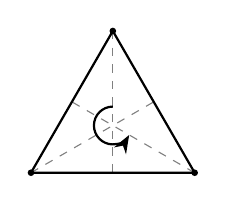
\begin{tikzpicture}[scale=0.8]
    % Define vertices of equilateral triangle
    \coordinate (A) at (90:1.5);
    \coordinate (B) at (210:1.5);
    \coordinate (C) at (330:1.5);
    
    % Define midpoints for reflection lines
    \coordinate (MA) at ($(B)!0.5!(C)$);
    \coordinate (MB) at ($(A)!0.5!(C)$);
    \coordinate (MC) at ($(A)!0.5!(B)$);
    
    % Draw reflection lines (dashed)
    \draw[dashed, gray] (A) -- (MA);
    \draw[dashed, gray] (B) -- (MB);
    \draw[dashed, gray] (C) -- (MC);
    
    % Draw the triangle
    \draw[thick] (A) -- (B) -- (C) -- cycle;
    
    % Draw vertices as dots
    \fill (A) circle (1.5pt);
    \fill (B) circle (1.5pt);
    \fill (C) circle (1.5pt);
    
    % Draw rotation arrow in center
    \draw[-{Stealth}, thick] (0,0.3) arc (90:330:0.3);
\end{tikzpicture}
\end{center}

Symmetires, then, permute the certices, and every permutation of the set of vertices arises from exacly one symmetry. Thus, \( S_{3} \) occurs as the group of symmetries of a triangle. The other groups in \( \mathbb{R}^2 \) that arise from symmetries are called dihedral groups, and the groups comprised of symmetries in \( \RR[3] \) are called octahedral groups. We will return to these at a later point. 

}

\ex{Matrix groups}{We have some special type of matrix groups, it is okay if you do not know much about them at the moment, we will dive into detail about them later; note that the following groups are all using the LOC of matrix multiplication. The first such group is the \textbf{\textit{general linear group}} given by \( \text{GL}_n(\mathbb{R}) \coloneqq \{\text{inverstible \( n \times n \) matrices with real coefficients}\}  \), the second is known as the \textbf{\textit{special linear group}} given by \( \text{SL}_n (\mathbb{R})\coloneqq \{n\times n \text{ real matrices with determinant }1\}  \), there also exists these for \( \CC \), and in fact for any \( \FF \) as we will later show from \( \GL(n,\FF) \) (you do not need to know what this means for now).} 


A group that has the property of being generated by an element (in example 2.0.3, the element that generates is a single symmetry) such that the entire group can be obtained by adding said element and/ or its inverse to itself repeatedly is said to be \textbf{\textit{cyclic}}. 



\section{Constructions}
A natural question that arises in the course of group study asks, \textit{how can we construct new groups from existing groups?} That is to say, how can one \textit{combine} groups? We combine groups using \textit{products} given by \( G \times H \) such that \( G,H \) are both groups; the underlying set is given by ordinary Cartesian product, and the law of composition is said to be given termwise; i.e.,
\[
  (a,b)\cdot (a',b')\coloneqq (aa',bb')
.\] 

There are times we may use the term \textit{sum} for the combination of \( G \) and \( H \), written \( G \oplus H \), but we usually have more specific uses for this term (though this may not \textit{always} be the case). For construction on more than two groups we simply have 
\[
  G_{1}\times \ldots G_n \coloneqq \{(a_{1},\ldots ,a_n)\mid a_i \in G_i\}  
\] with LOC given by \[
(a_{1},\ldots ,a_n)\cdot (b_{1},\ldots, b_n)\coloneqq (a_{1}b_{1},\ldots ,a_nb_n)
.\] When taking the product of \( n \) groups (i.e., \( G^n \) (e.g., \( \mathbb{Z}^n \))) we usually denote this via 
\[
  \bigoplus^n_{i=1}G_i \text{ or } \prod_{i=1}^{n}G_i
.\] 

When given infinitely many groups, our summation symbol takes on a special property,
wherein \( \prod_{i=1}^{\infty} G_i=\{(a_{1},a_{2},\ldots )\mid a_i \in  G_i\}  \), but \( \bigoplus_{i=1}^{\infty}G_i=\{(a_{1},\ldots )\mid a_i \in G_i, \text{ where all but finitely many \( a_i \) are identity}\}  \). We can see this best exemplified with some polynomials:

\ex{Power series and polynomial groups}{Consider \( G_{0}=G_{1}=\ldots =(\mathbb{R},+) \) for \( (a_{0},a_{1},\ldots ) \) by \( \sum^n_i a_ix^i \), then
\[
   \prod^{\infty}_{i=0}\mathbb{R}=\mathbb{R}[[x]], \text{ i.e., formal power series } \sum_{i=0}^{\infty}a_ix^i \text{ under addition} 
,\] 
and 
\[
\bigoplus^{\infty}_{i=0}\mathbb{R}=\mathbb{R}[x], \text{ i.e., polynomials } \sum_{\text{finite}}a_ix^i
.\]} 

\section{Subgroups and Homomorphisms} 
Similar to how we have had subsets, we, too, have \textbf{\textit{subgroups}}!

\dfn{Subgroups and proper subgroups}{A \textbf{\textit{subgroup}} \( H\) of \( G \) is a non-empty subset \( H\subset G \) which is closed under the given law of composition---that is to say, \( \forall a,b \in H \implies ab \in H \)---and inversion---i.e., \( \forall a \in H \implies a^{-1}\in H \). Since \( H \neq \emptyset \), those 2 conditions imply \( e \in H \). Thus \( H \) under the same operation as \( G \) is a group within its own right. We say that \( H \) is a \textbf{\textit{proper subgroup}} if \( H \subset G \) but \( H\neq G \).}

\thm{}{Let \( S \) be a subgroup of \( (\mathbb{Z},+) \) (somtimes represented as \( \mathbb{Z}^+ \)). Either \( S=\{0\}   \)---the trivial subgroup---or it is the form \( \mathbb{Z}a \) such that \( a \) is the smallest positive integer in \( S \).}
\pf{Proof}{Refer to Artin Ch.2, Thm.2.3.3.}
\mprop{Title}{Let \( a,b \in \mathbb{Z} \), not both zero, and let \( d \) be their greatest common divisor, the positive integer that generates the subgroup \( S=\mathbb{Z}a+\mathbb{Z}b \). So \( \mathbb{Z}d=\mathbb{Z}a+\mathbb{Z}b \). Then 
  \begin{enumerate}[(a)]
  \item \( d \) divides \( a \) and \( b \);
  \item if an integer \( n \) divides both \( a \) and \( b \), it, too, divides \( d \);
  \item there are integers \( r \) and \( s \) such that \( d=ra+sb \).
\end{enumerate}}
\cor{}{A pair \( a,b \in \mathbb{Z} \) is relatively prime \( \iff \) there are integers \( r \) and \( s \) such that \( ra+sb=1 \).}
\cor{}{Let \( p \in \PP \). If \( p \) divides a product of \( ab \in \mathbb{Z} \), then \( p \) divides \( a \) XOR \( p \) divides \( b \).}

\dfn{Homomorphisms and isomorphisms}{Given two groups \( G,H\), a \textbf{\textit{homomorphism}} (abbr. homom. or hom.) \( \varphi : G \to H \) is a map which respects the law of composition and is such that \( \forall a,b \in G, \varphi (ab)=\varphi (a)\varphi (b) \). This implies \( \varphi (e_G)=e_H \) and \( \varphi (a\inv )=\varphi (a)\inv \). An \textbf{\textit{isomorphism}} (abbr. isom.) is a bijective homomorphism. If \( G \) and \( H \) are isomorphic, they are essentially the "same" group structure-wise, even if its elemnts and laws may have different names!}




% Your notes here...

% ============================================================
% lecture_03
% ============================================================

\lecture{3}{Group Relations}

\section{Symmetry Group}

\section{Group Relations}

\subsection{Subgroups}
\subsection{Homomorphisms}
\subsection{Kernals, Images, and Order}
\subsection{Finite Symmetric Groups}

% Your notes here...

% ============================================================
% lecture_04
% ============================================================

\lecture{4}{Quotient Groups}

\section{Cardinality}
\section{Sets of Maps and Powersets}
\section{Equivalence Relations}
\section{Quotient Groups}
\section{Congruence mod \( H \)}


% Your notes here...

\end{document}
